\section{Design for Learning}

%\citepp{effectivelearning-robert}
%\citepp{learning-krathwohl}
%\citepp{learning-ucla}

The following sections deals with how to design for effective learning \citep{dirksen}. Designing for the mind is sometimes referred to as cognitive psychology, how our brain works in regard to mental processes such as retention and transfer of knowledge. There are a number of strategies and techniques that can be used when designing \textit{learning} for the mind specifically: to decide educational objectives, how to reach these objectives (building skills and learning from assessment), and how to retain information (learning by reflection).
 % Design for How People Learn (book, torrent)

%On January 28th, 2016, Henrik Marklund\ref{effectivelearning-expert} at the educautional technology startup Knowly was interviewed about Pedagogic Development. He means there are two main areas of research, and an additional one.
%The third area, training transfer, is the research on how to make sure a course gives effect in everyday life.

%The third area is training transfer, and asks "How do you make sure a course gives effect in your everyday life?". For YoungDrive, the wish is that the coach training gives effect in the coaches' everyday life. The master thesis aims to be able to assess and encourage this.

%\subsection{Pedagogical development}

%The first section describes "How do you get people to learn things?", cognitive psychology. Often school is studied, where learning is about being taught a subject, and then to pass a test. E-learning tools are often designed to do similar things to what schools does.

%The second section describes "How do you get people to behave differently?", social psychology. One area of research is about building habits. This is highly relevant in e-learning, where behavior change may be necessary to build the habit of using an app or a digital tool repeatedly.

%\include{theory/learning/pedagogical-development/cognitive_psychology}

%\subsubsubsection{Learning}

  \subsection{Learning Entrepreneurship: Mapping Educational Objectives with Bloom's Revised Taxonomy}

  What to teach should be determined by the learning objectives of the activity. Learning activities often involve both lower order and higher order thinking skills as well as a mix of concrete and abstract knowledge. All of this needs to be designed for depending on activity. Bloom's Revised Taxonomy \citep{krathwohl} separates between lower or higher cognitive complexity, and concrete (factual or conceptual) or abstract knowledge (procedural or metacognitive) \citep{cheong}. The taxonomy thus provides a framework for determining and clarifying learning objectives. Bloom's Revised Taxonomy is useful to map the whole range of learning objectives for entrepreneurship and as an entrepreneurship coach. See figure \ref{fig:revised-bloom} from \cite{heer}. Each colored block is an example of a learning objective matching with the two dimensions. The figure also explains the different concepts. Depending on the objective, it fits differently into the Knowledge dimension and Cognitive Process dimension of Bloom's Revised Taxonomy.

  \begin{figure}[h]
    \centering
    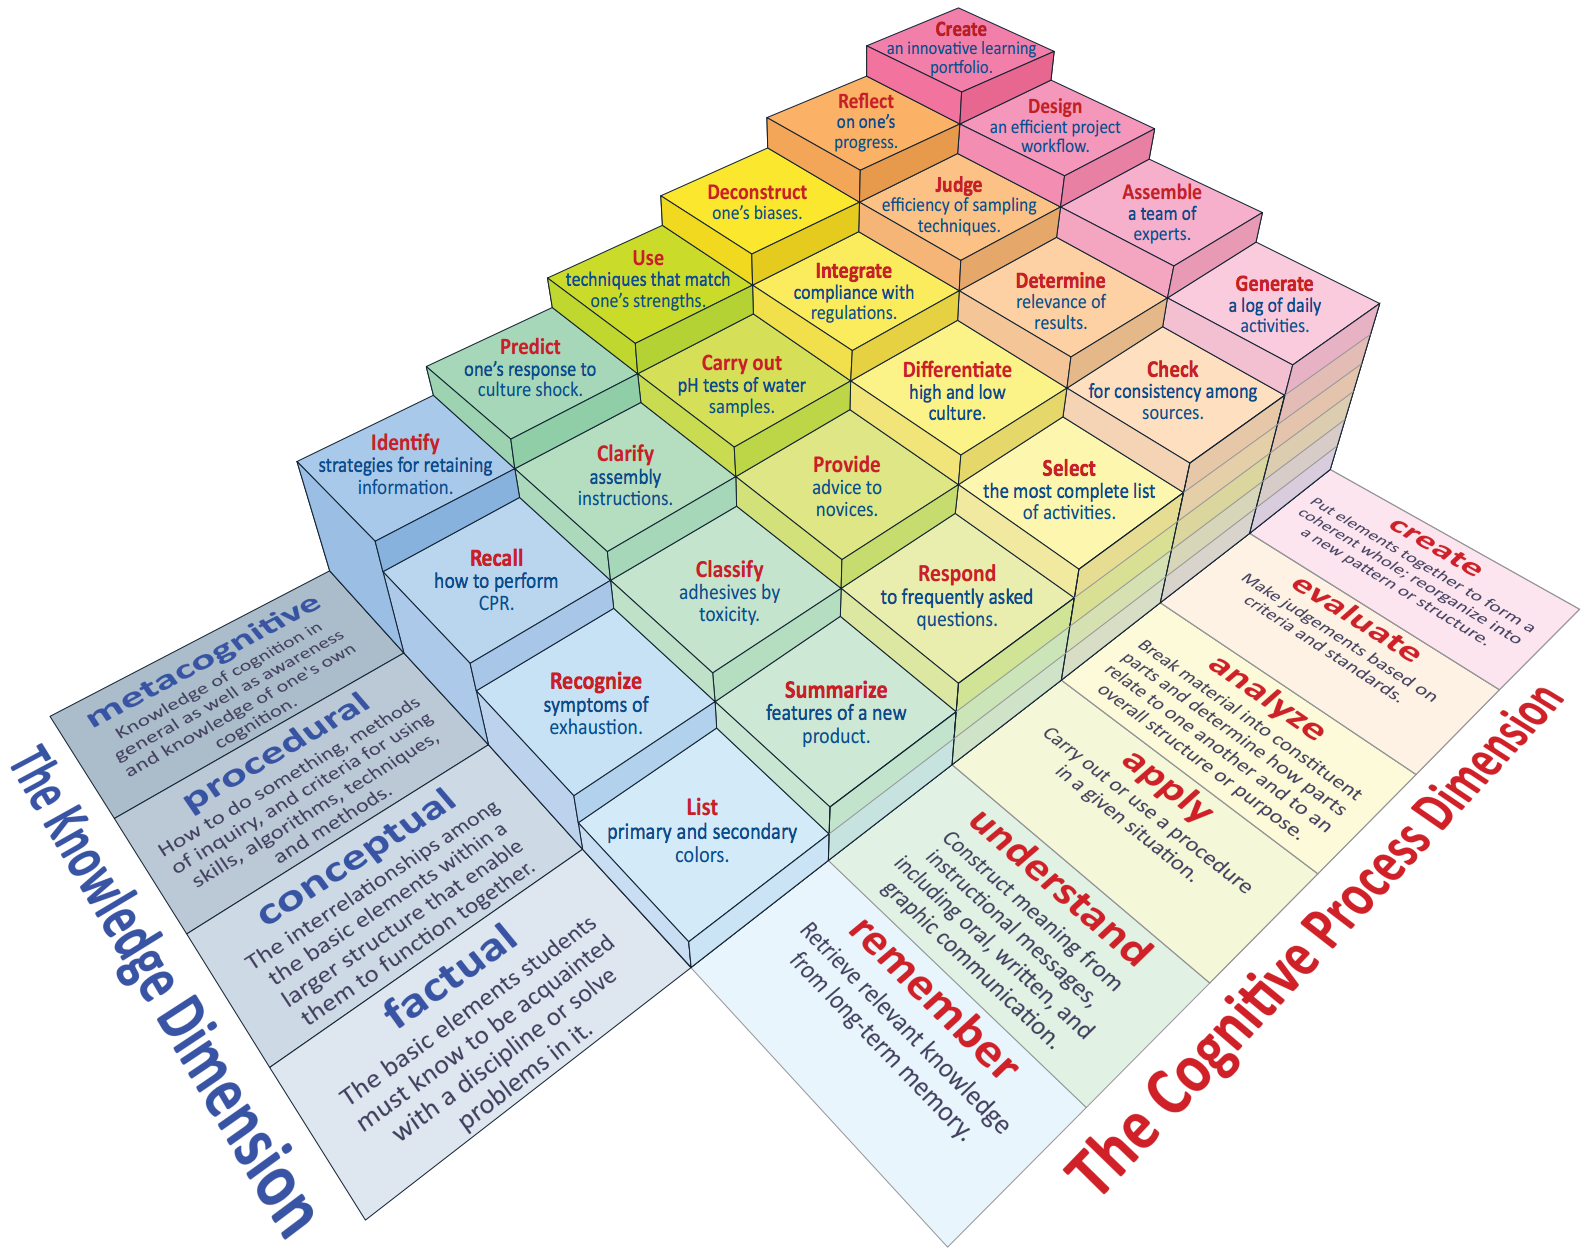
\includegraphics[width=1.0\textwidth]{RevisedBloom.png}
    \caption{Bloom's Revised Taxonomy visualised with examples of different learning objectives. The entrepreneurship topic question "What is financial literacy?" would be \textit{conceptual} and \textit{remember}. }
    \label{fig:revised-bloom}
\end{figure}

  To craft good multiple-choice questions could be an art, but to map the question to learning objective makes it into more of a science: when designing for learning, using Bloom's Revised Taxonomy you can analyse if the educational objectives are met.

  \subsection{Building Skills: by Spaced Practice, Deliberate Practice and Perceptual Exposure}

  Spaced practice deals with spreading out learning, with the purpose of improving retention. \cite{gates} concludes that spaced learning versus massed learning (no rest between sessions) did have a memory benefit in their study, and found no evidence of consistent correlation between total duration and effects on learning outcomes in their study. Taking spaced learning into consideration, could mean making the user apparent on the person's meta-cognitive ability (your personal insight of what you'll remember and when you are likely to forget).

  To design for optimal learning outcomes of skills (e.g. entrepreneurial activity or coaching skills), deliberate practice has been proven effective. It has been tested before for mobile learning environments \citep{yengin}. Building skills effectively, \cite{sierra} suggests helping users practice right, by designing practice exercises that will take a fine-grained task from unreliable to 95\% reliability, within one to three 45-90-minute sessions. \cite{sierra} suggests skills to be divided into three buckets: can't do (but need to do), can do with effort, and mastered (reliable/automatic). The goal then is to move skills from can't do into mastered, in the best way possible. See figure \ref{fig:sierra-practice} from \cite{sierra}. If you can’t get the user to 95\% reliability within this time, stop trying; you need to redesign the sub-skill \citep{sierra}.

  \begin{figure}[h]
    \centering
    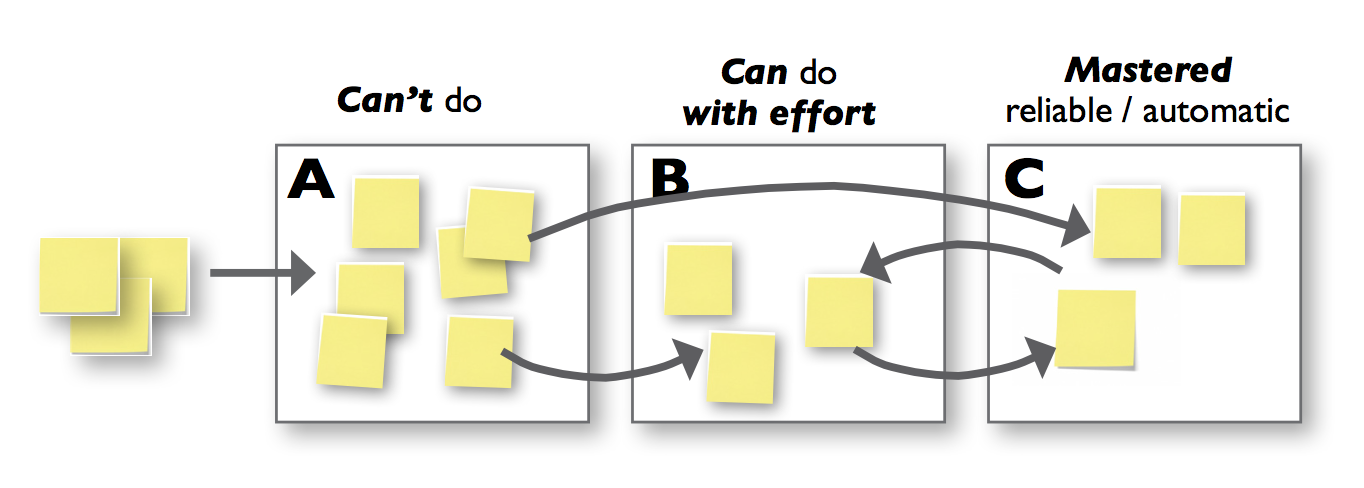
\includegraphics[width=0.8\textwidth]{SierraPractice.png}
    \caption{Moving skills from A (Can't do) to B (Can do with effort) into C (Mastered) can move different ways, depending on how effective the learning is. Deliberate practices focus on A-B-C, while perceptual expose enables A to C. Reflection allows knowledge to go backwards, to get better at the skill than previously possible. An example might be to teach "Financial literacy". Concepts and factual knowledge (like what income and profit is) might need to move A-B-C, whereas entrepreneurship skills (like taking financial decisions) can move A-C if it becomes intuitive for the user, e.g. via having been exposed to a lot of trial-and-error examples in the app.}
    \label{fig:sierra-practice}
  \end{figure}

  Desirable difficulties applies here, meaning that during deliberate practice, it may feel as if learning gets more and more difficult, but in the long term the user is actually learning more. As a result, fewer people does true deliberate practice, but they do not get the same reward in return. \cite{sierra} suggests motivation to overcome desirable difficulties, see section \ref{sec:motivation}.

  By deliberate practice, you can practice better. The second attribute of becoming an expert is being exposed to high quality, high quantity examples of expertise \citep{sierra}. It shows that whenever a skill relies on intuition, we could try exposing the user a well-designed trail and error test. In the case of multiple-choice questions, this could be done by exposing users to very high-quality samples during a very limited time. Perceptual knowledge includes teaching what we think of as expert intuition (like being a good entrepreneurship coach).

  Sierra shows how researchers have repeatedly, by well-designed tests, been able to quickly build expertise by trial-and-error feedback. A novice would hazard a guess and an expert would say yes or no. Eventually the novices became, like their mentors, masters of the expertise that could otherwise would have been intangible for long.

  \subsection{Learning from Assessment}\label{learning-assessment}

  Regarding assessment, knowing what learners know and don't know is crucial to effective learning, \cite{luckin} says. Assessment can partly help to design for flow, as assessment can help perfectly match the learner's ability with the given challenge \citep{bruhlmann}, which is effective for intrinsic motivation (see section \ref{sec:motivation}). Moreover, it also has cognitive benefits. It can help to offer appropriate feedback, increase learners' awareness of their learning needs, and give accurate assessment and analysis, and allows learning to be tailored.

  By recognizing differences between students, in their ability to understand what they know and how they can progress, it is possible to ensure that everyone achieves their full potential. Effective assessment by a teacher or agent includes individual feedback (task-oriented and informal) and appropriate feed-forward advice. \cite{sitzmann} has studied how questions used to prompt self-monitoring and self-evaluation benefit learning, showing gradual, positive  effect on learning. Regarding multiple-choice tests, \cite{nicol} gives seven principles of good feedback practice, see figure \ref{fig:multiple-choice}.

  \begin{figure}[h]
    \centering
    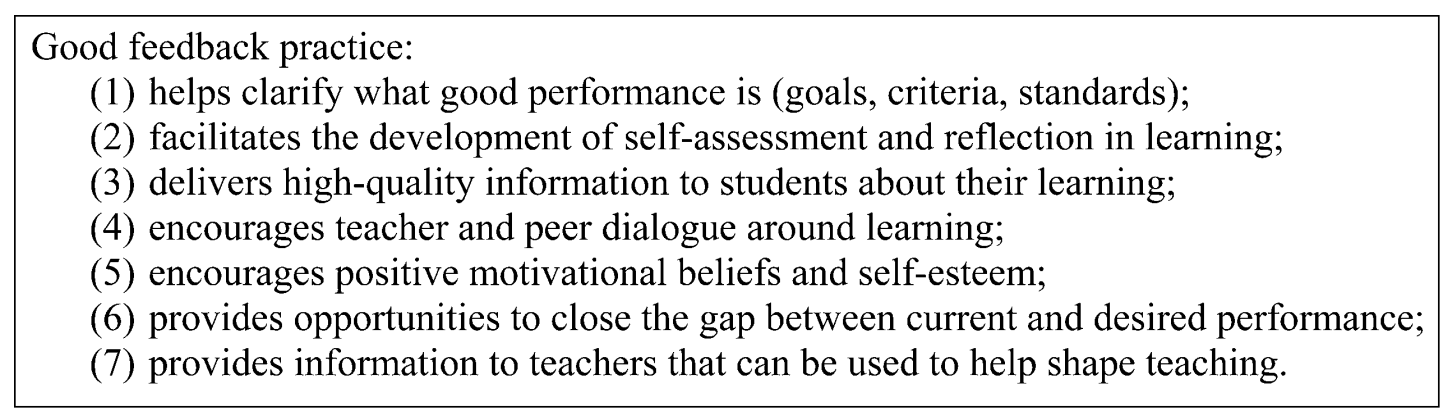
\includegraphics[width=0.8\textwidth]{multipleChoice.png}
    \caption{Seven principles of good feedback practice \cite{nicol}.}
    \label{fig:multiple-choice}
\end{figure}

  Moreover, research on fixed mindset (I can't do X) versus growth mindset (I can't do X \textit{yet}) talks about how mindset guides behaviour. In a mathematics game students were rewarded by the mentality of "Not yet" and effort versus getting a grade on existing knowledge \citep{dweck}. Regarding learning, those exposed to a growth mindset mentality, previously having a fixed mindset, got superior results, especially those students previously having difficulties with learning. Regarding motivation, a study showed that high achievers played to the end regardless, but in the growth mindset version those still played to the end, but so many more lower and medium achievers also stayed until the end \citep{dweck}.

  \subsection{Learning by Thinking: Reflection \& Retrieval Practice}\label{learningbythinking}

  \cite{stefano} suggests that in some cases, learning from reflection is more effective than learning by doing. During the act of reflection, the student develops necessary skills and self-awareness to refine their own learning activities. His results suggest that reflection as an activity that can be more effective than additional learning. This surely applies to the teacher as well says \cite{luckin}. \cite{stefano} found that individuals who are given time to reflect on a task, outperforms students who are given the same amount of time to practice with the same task. But, similar to deliberate practice, it is a desirable difficulty: individuals in the test themselves, had a tendency to believe that allocating time to practice on the task rather than reflecting on it would benefit them.

  %\subsection{Retrieval practice}

  When it comes to study technique, \cite{bjork} as well shows that retrieval from memory is more effective than people who repeat reading the same thing to remember: the more effective students, retrieves from memory. One way to use memory retrieval as a study technique, is to ask "What was in that article?", before checking the answer in the article (the flashcard principle). It is an example of memory retrieval that is extremely effective for learning, their research shows. There is a danger with multiple-choice questions, that the student is given no time to reflect on the question and their prior knowledge, before evaluating the alternatives \citep{nicol}. In the case of learning to teach entrepreneurship, where the information should be easily accessible during the teaching situation, selecting an alternative from multiple-choice does not simulate the teaching environment. Thus, memory via retrieval is essential in the multiple-choice design to have an effect in a real-world teaching scenario.

%\subsection{Not forgetting}

%UCLA Bjork's Learning and Forgetting Lab researches how people forget, and how to design so that people do not forget.

%\include{theory/learning/pedagogical-development/social_psychology}
